\documentclass{report}
\usepackage[utf8]{inputenc}
\usepackage{xcolor}
\usepackage{url}
\usepackage[nottoc]{tocbibind}
\usepackage{graphicx}
\usepackage[bottom]{footmisc}
 

\title{Project Document: Team Name}
\author{Team Member 1 \\
Team Member 2 \\
Team Member 3 }
\date{}

\begin{document}

\maketitle

\tableofcontents

\begin{abstract}
This is the template you are required to use for your project milestone write-ups.  Each submission will build on the previous one.  At this spot in your report, you should place a brief abstract (4--6 sentences). This is a high-level summary of your work, including a brief summary of the problem, motivation, and your results.  Since your work will evolve for each milestone, the abstract should get updated with each submission.
\end{abstract}

\chapter{Milestone 1: Project Ideas}

\section{Introduction}

Here you should give an 
overview of your process, where you looked for project ideas. Citations are important. 

A few other notes, since I have your attention. First, you should be using figures and/or tables, especially in later milestones with experimental results.  If you have no tables or figures to summarize experimental results, then something is very, very wrong. 

Second, you {\bf must} refer to your figures and tables in the main text, and summarize/explain each of  them.  Each figure/table {\bf must have a caption}.  Table captions go {\bf above} the table, and figure captions go {\bf below} the figure\footnote{I don't make the rules, but I will enforce them.}. 

For example, Figure~\ref{fig:compute} shows how computing power requirements for cutting-edge deep learning projects have increased over time. At this point, we would maybe point out a few interesting things, like how quickly it increases after 2011. Then, for a completely unrelated note in the same paragraph\footnote{Don't do this!}, Table~\ref{tab:CNN-perf} summarizes  performance of various CNN architectures on ImageNet.  Here we could point out how quickly the error rates drop. 

\begin{figure}
    \centering
    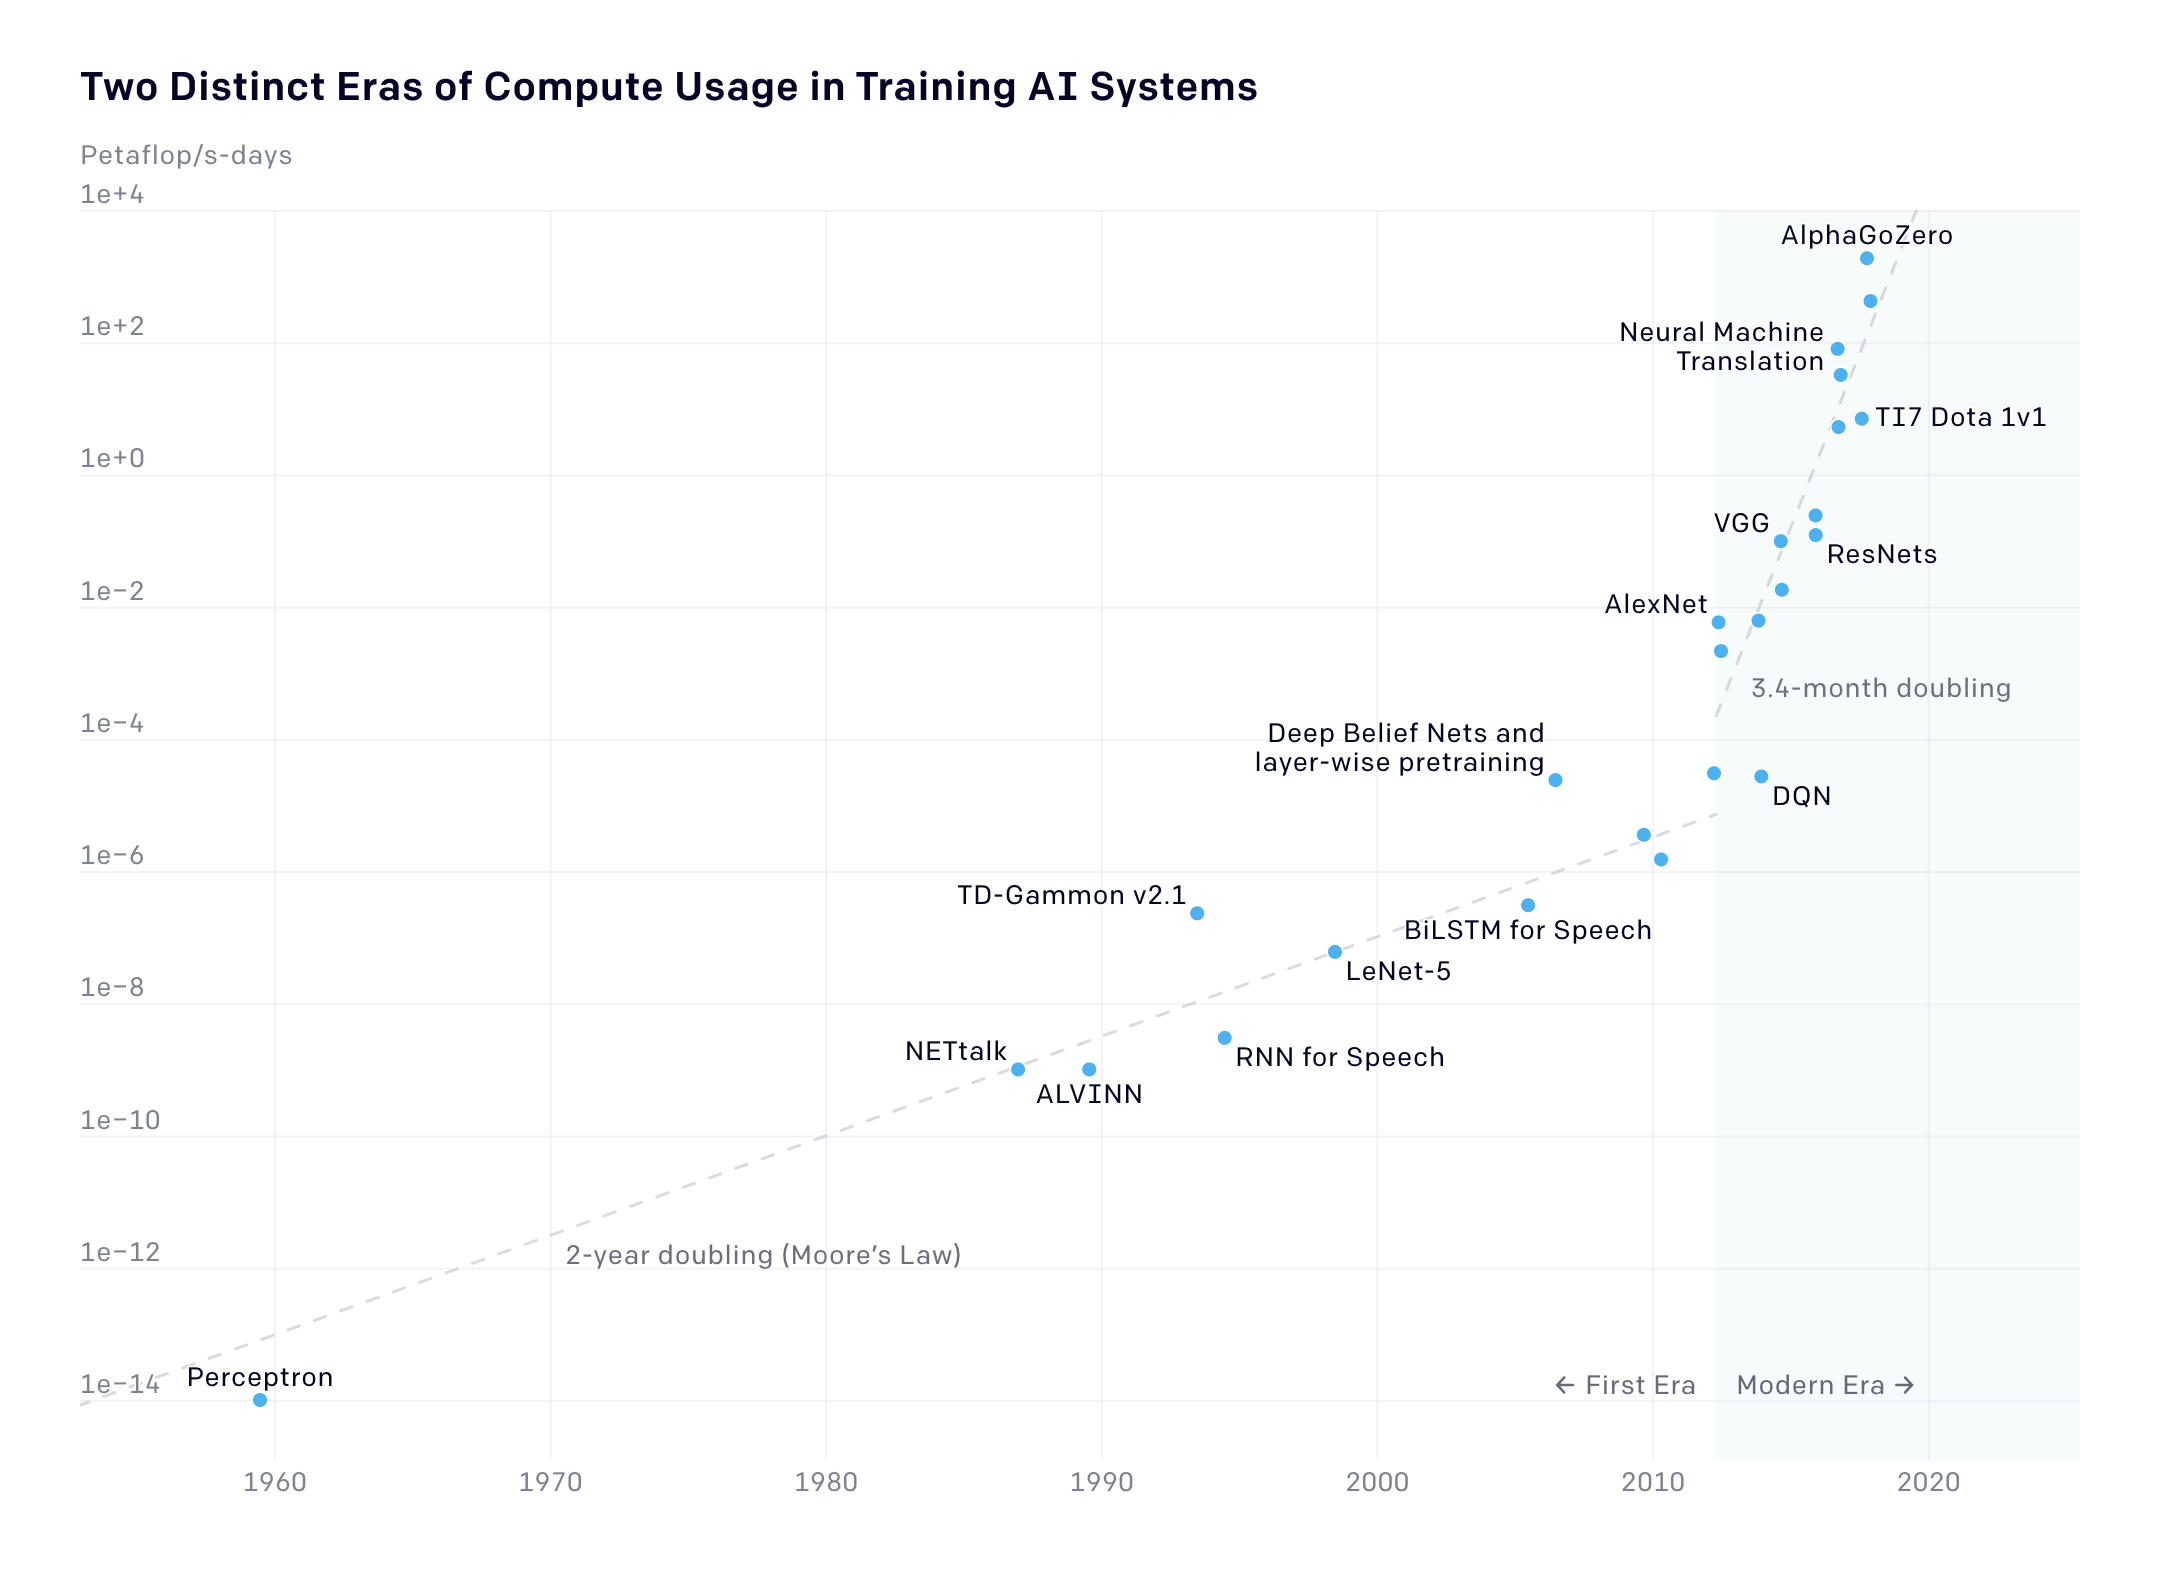
\includegraphics[width=\textwidth]{figs/ai-and-compute-all-2.png}
    \caption{Compute for cutting-edge deep learning projects vs.\ time (source:~\cite{AI-compute18}).}
    \label{fig:compute}
\end{figure}

\begin{table}[]
    \centering \caption{Top-5 error on ImageNet for various convolutional architectures.}
    \begin{tabular}{|c|c|c|} \hline
      Architecture   &  Year & Top-5 Error \\ \hline
    AlexNet & 2012     & 17\% \\
    GoogLeNet & 2014 & 7\% \\
    ResNet & 2015 & 3.6\% \\ \hline
    \end{tabular}
 
    \label{tab:CNN-perf}
\end{table}

\section{Project Idea 1: [name]}

Summarize the problem, list applications, summarize approaches to this problem. 


\section{Project Idea 2: [name]}

Summarize the problem, list applications, summarize approaches to this problem 

\section{Conclusions}

Sum up your results, including your opinion on each project idea.  Also, list any questions that you have for the instructor and TA regarding your project work.

\textcolor{red}{Remember to cite sources using BiBTeX and add those references to the end of this document!}

It is okay to cite some websites and tutorials (if you first look up how to properly cite them!), but you must also cite some refereed publications from conferences and/or journals.

Sample citation~\cite{Samuel59}

\chapter{Milestone 2: Project Selection}

In this chapter, you should select your project, formally define it, and propose two approaches, each with a work plan.  You should follow the The Heilmeier Catechism~\cite{heilmeier}, which is a set of questions used to evaluate proposed research programs:  
\begin{enumerate}
    \item What are you trying to do? Articulate your objectives using absolutely no jargon.
   \item How is it done today, and what are the limits of current practice?
   \item What is new in your approach and why do you think it will be successful?
   \item Who cares? If you are successful, what difference will it make?
   \item What are the risks?
   \item How much will it cost?
   \item How long will it take?
   \item What are the mid-term and final ``exams'' to check for success?
\end{enumerate}

\section{Introduction}

Explain which project you chose, and why. (This can differ from the two you proposed in the previous chapter.) 

\section{Problem Specification}

Formally define your chosen problem, including the following, as subsections:
\begin{enumerate}
    \item A brief statement of your project topic (HC1).
    \item Motivation for your topic: why it is important and interesting (HC3, HC4). If your work is in an application area, be careful to avoid technical jargon from that area that is outside of computer science. If you must use a term, define it as carefully and simply as possible.
   \item What resources will you need, including data sets and libraries that need to be installed on {\tt crane} (HC6).
   \item Cite at least three references (at least two published journal or conference papers) (HC2).
\end{enumerate}

\section{Proposed Method 1: [name]}

Propose a step-by-step approach to solve your chosen problem.  You should include 
a precise work plan: what you plan to do, what data sets you will test on, how you will preprocess the data, what the steps (pipeline) of this method (e.g., what NN architecture(s) will be used and how they'll be linked), how you will evaluate performance, what is your timeline, etc.\ (HC5, HC7, HC8).  One or more of your references should relate to aspects of this. 


\section{Proposed Method 2: [name]}

Propose a step-by-step approach to solve your chosen problem.  You should include 
a precise work plan: what you plan to do, what data sets you will test on, how you will preprocess the data, what the steps (pipeline) of this method (e.g., what NN architecture(s) will be used and how they'll be linked), how you will evaluate performance, what is your timeline, etc.\ (HC5, HC7, HC8).  One or more of your references should relate to aspects of this. 

\section{Conclusions}

Sum up, including your opinion on each approach.  Also, list any questions that you have for the instructor and TA regarding your project work.

\textcolor{red}{Remember to cite sources using BiBTeX and add those references to the end of this document!}

It is okay to cite some websites and tutorials (if you first look up how to properly cite them!), but you must also cite some refereed publications from conferences and/or journals.

\chapter{Milestone 3: Progress Report 1}

\section{Introduction}
\label{sec:M3-intro}

Remind the reader of the problem you're working on, and what your approach is.  Briefly summarize what your results are so far.

\section{Experimental Setup}
\label{sec:M3-setup}

Describe the setup of your experiments so far in sufficient detail for the reader to reproduce them.  Include data sources, preprocessing used, architectures/other approaches used, hyperparameter values used, performance measures used, other relevant items (e.g., cross-validation).

\section{Experimental Results}
\label{sec:M3-results}

Present your results so far using tables, figures, confusion matrices, etc.\ (whatever is appropriate). 

\section{Discussion}

Discuss your experimental results, drawing conclusions that are supported by your experimental results of Section~\ref{sec:M3-results}.  Be careful to not draw conclusions that are not supported by the evidence you present! Discuss how these results will influence your future experiments.

\section{Conclusion}

Sum up, including your a summary of your results so far (recapitulating that from Section~\ref{sec:M3-intro}).  Also, describe your plans for future work and list any questions that you have for the instructor and TA regarding your project work.

\textcolor{red}{Remember to cite sources using BiBTeX and add those references to the end of this document!}

It is okay to cite some websites and tutorials (if you first look up how to properly cite them!), but you must also cite some refereed publications from conferences and/or journals.


\chapter{Milestone 4: Progress Report 2}


\section{Introduction}
\label{sec:M4-intro}

Remind the reader of the problem you're working on, and what your approach is.  Briefly summarize what your results are so far.

\section{Experimental Setup}
\label{sec:M3-setup}

Describe the setup of your experiments so far in sufficient detail for the reader to reproduce them.  Include data sources, preprocessing used, architectures/other approaches used, hyperparameter values used, performance measures used, other relevant items (e.g., cross-validation).

\section{Experimental Results}
\label{sec:M4-results}

Present your results so far using tables, figures, confusion matrices, etc.\ (whatever is appropriate). 

\section{Discussion}

Discuss your experimental results, drawing conclusions that are supported by your experimental results of Section~\ref{sec:M4-results}.  Be careful to not draw conclusions that are not supported by the evidence you present! Discuss how these results will influence your future experiments.

\section{Conclusion}

Sum up, including your a summary of your results so far (recapitulating that from Section~\ref{sec:M4-intro}).  Also, describe your plans for future work and list any questions that you have for the instructor and TA regarding your project work.

\textcolor{red}{Remember to cite sources using BiBTeX and add those references to the end of this document!}

It is okay to cite some websites and tutorials (if you first look up how to properly cite them!), but you must also cite some refereed publications from conferences and/or journals.



\chapter{Milestone 5: Final Report}


\section{Introduction}
\label{sec:M5-intro}

Remind the reader of the problem you're working on, and what your approach is.  Briefly summarize what your final results are.

\section{Experimental Setup}
\label{sec:M3-setup}

Describe the setup of your experiments  in sufficient detail for the reader to reproduce them.  Include data sources, preprocessing used, architectures/other approaches used, hyperparameter values used, performance measures used, other relevant items (e.g., cross-validation).

\section{Experimental Results}
\label{sec:M5-results}

Present your results  using tables, figures, confusion matrices, etc.\ (whatever is appropriate). 

\section{Discussion}

Discuss your experimental results, drawing conclusions that are supported by your experimental results of Section~\ref{sec:M5-results}.   Be careful to not draw conclusions that are not supported by the evidence you present!

\section{Conclusion}

Sum up, including your a summary of your results  (recapitulating that from Section~\ref{sec:M5-intro}).  Also, describe possible avenues for future work (should one continue the project) and list any questions that you have for the instructor and TA regarding your project work.

\textcolor{red}{Remember to cite sources using BiBTeX and add those references to the end of this document!}

It is okay to cite some websites and tutorials (if you first look up how to properly cite them!), but you must also cite some refereed publications from conferences and/or journals.

\appendix

\chapter{First Appendix}

An appendix is used only if necessary (remove this chapter if you don't use one). It contains supplementary materials/extra details such as extensive experimental results (e.g., hyperparameter search results, where the most interesting ones are in the main text and the rest are dumped here), detailed proofs, etc. 

Create as many appendices as needed by adding chapters. All such chapters must be before the bibliography. 


\bibliographystyle{plainurl}
\bibliography{main}

\end{document}
